\chapter{Hardware Implementation}
\label{chap:2}
In this chapter we describe the hardware implementation of the system. In particular, in section \ref{sec:turret12} and \ref{sec:turret64} we will focus on the two different laser turrets built, pointing out all the issues and differences that make the second one better. We also mention the arm IMU device and the groud robot used for reconstruct human pointing and build our demos respectively.
\section{First Turret Model} \label{sec:turret12}
Figures \ref{fig:firstModelSide} (SCATTARE IMMAGINI MIGLIORI) shows the first turret. As we can see, it follows the model already seen in chapter \ref{chap:1}. So, at the base we have one servo motor in charge to control the \emph{pan} angle. On its flange, a second motor is mounted with a plastic bracket on its own flange. The laser diode is then mounted in the middle of that bracket, in such a way that its direction passes through the middle of the servo shaft. So, the second servo directly controls the \emph{tilt} angle. 
The \emph{Arduino Uno Board} and the \emph{Bioloid Bus Serial Interface} conclude our hardware list.
\\In the next sections we analyze each parts and their uses in details.
\begin{figure}
	\centering
	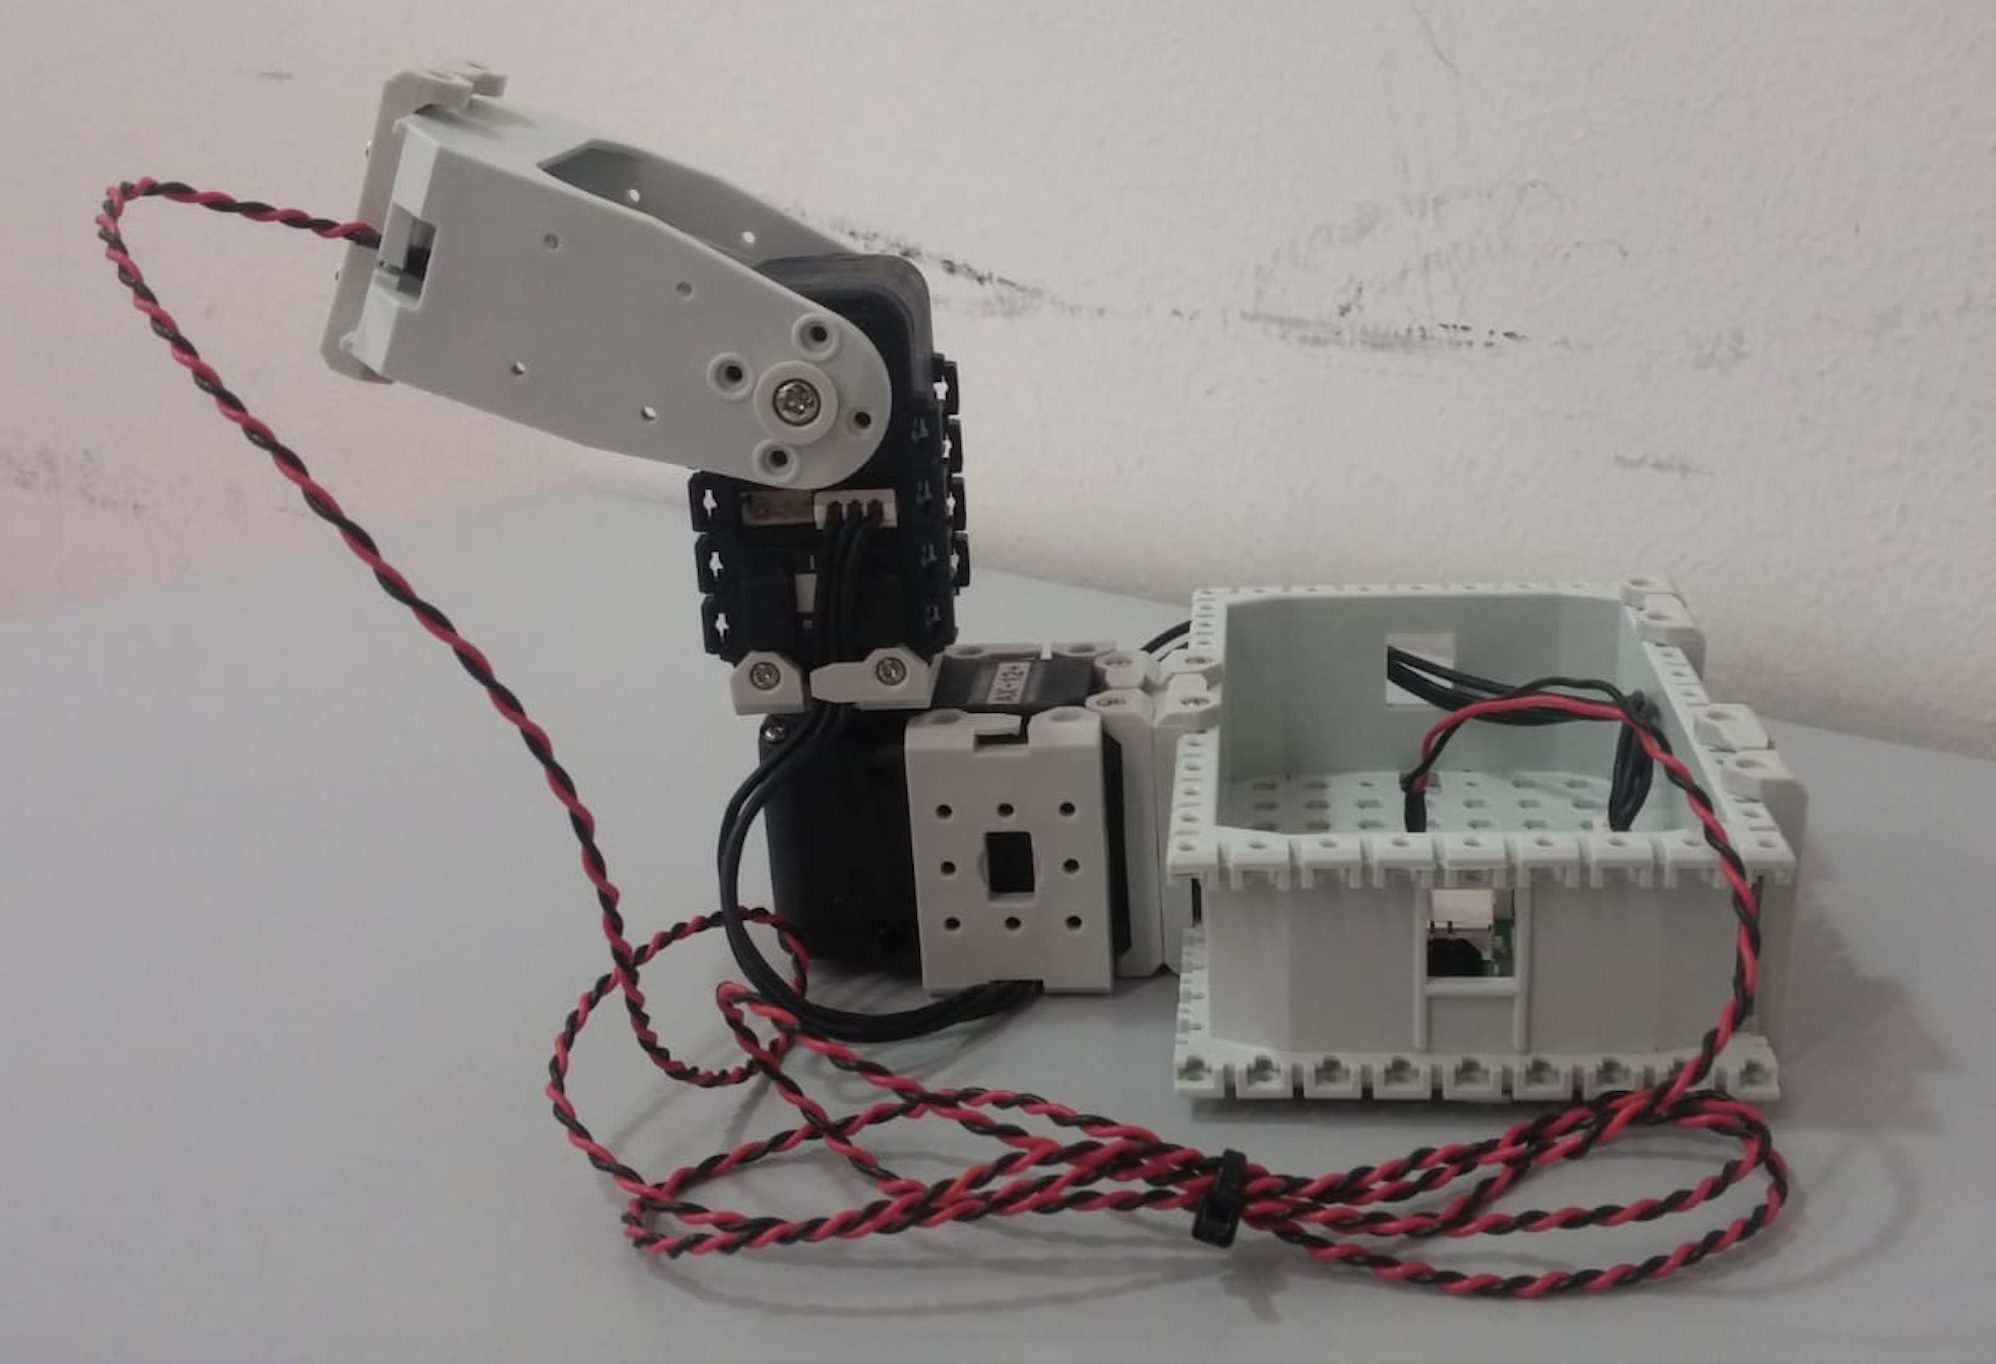
\includegraphics[width=\textwidth]{img/firstModelSide.png}%
	\caption{First Turret Model, Side}
	\label{fig:firstModelSide}
\end{figure}
\subsection{Dynamixel AX-12+}
As reported on the official website \cite{web-AX-12}:\\ \virgolette{\emph{the DYNAMIXEL is a smart actuator system developed to be the exclusive connecting joints on a robot or mechanical structure. DYNAMIXELS’ are designed to be modular and daisy chained on any robot or mechanical design for powerful and flexible robotic movements. The DYNAMIXEL is a high performance actuator with a fully integrated DC (Direct Current) Motor + Reduction Gearhead + Controller + Driver + Network, all in one servo module actuator. Programmable and networkable, actuator status can be read and monitored through a data packet stream.}}\\
The first turret is composed of two \textbf{Dynamixel AX-12+} motors.
\subsection{Motor Specification}
The full datasheet can be found here \cite{datasheet-AX-12}. We are mostly interested in two specifications: 
\begin{itemize}
    \item \textbf{Resolution}: $0.29^{\circ}$;
    \item \textbf{Communication speed}: 7343 bps $\sim$ 1 Mbps.
\end{itemize}
Those are the values that set the limitations for that turret, causing the issues we discuss in the next section.
\begin{figure}
	\centering
	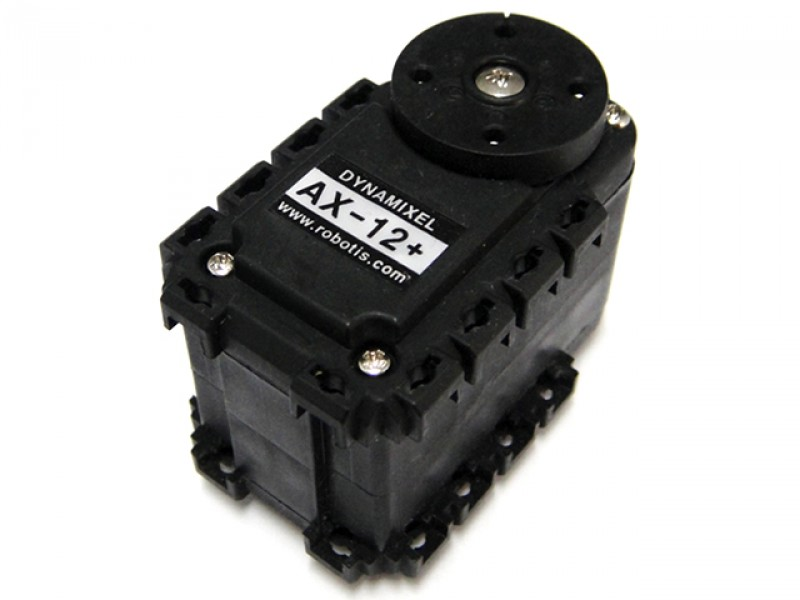
\includegraphics[width=0.5\textwidth]{img/ax12+.jpg}%
	\caption{Dynamixel AX-12+}
	\label{fig:ax12+}
\end{figure}
\subsection{Issues}\label{subs:firstModel:issues}
Here we will only report the issues raised by the motors. Solutions are discussed in the next chapter.
\subsubsection{Servo Resolution and Slow Speed Limit}
Even though a resolution of $0.29^{\circ}$ could seem pretty good, that value heavily limits the performance of the turret. As a matter of fact, in our system, the joint will be often asked to do very small movement and, thus, drawing tiny angles. Moreover, the motor is not able to move with too much low speed values. That issue becomes even bigger when the laser dot moves far from the turret: the angles become always more smaller. The result is that the performances of the turret can be good enough only on a small size space around the turret, but that is not certainly enough for our system.
\subsubsection{Trajectory Smoothness}
The performances degradation heavily impacts the smoothness of trajectory of the laser dot. Playing with servos internal parameters we could try to find the right trade-off between precision and smoothness, but since the relative localization is based on the laser positions and the user following those positions, then we can not sacrifice either precision or smoothness.
\subsubsection{Slow Communication Protocol}
This is the main issue. This is only partially related with the communication speed of the motors. Of course, with a higher speed, we could afford to use a slower protocol. Anyway, solving that issue allows us to obtain the best from that turret, hitting its limits, but obtaining a system which could work well enough for our purposes. Since the solution is part of the software implementation, it will be presented in the next chapter.

\subsection{Bioloid Bus Interface}
\begin{figure}
	\centering
	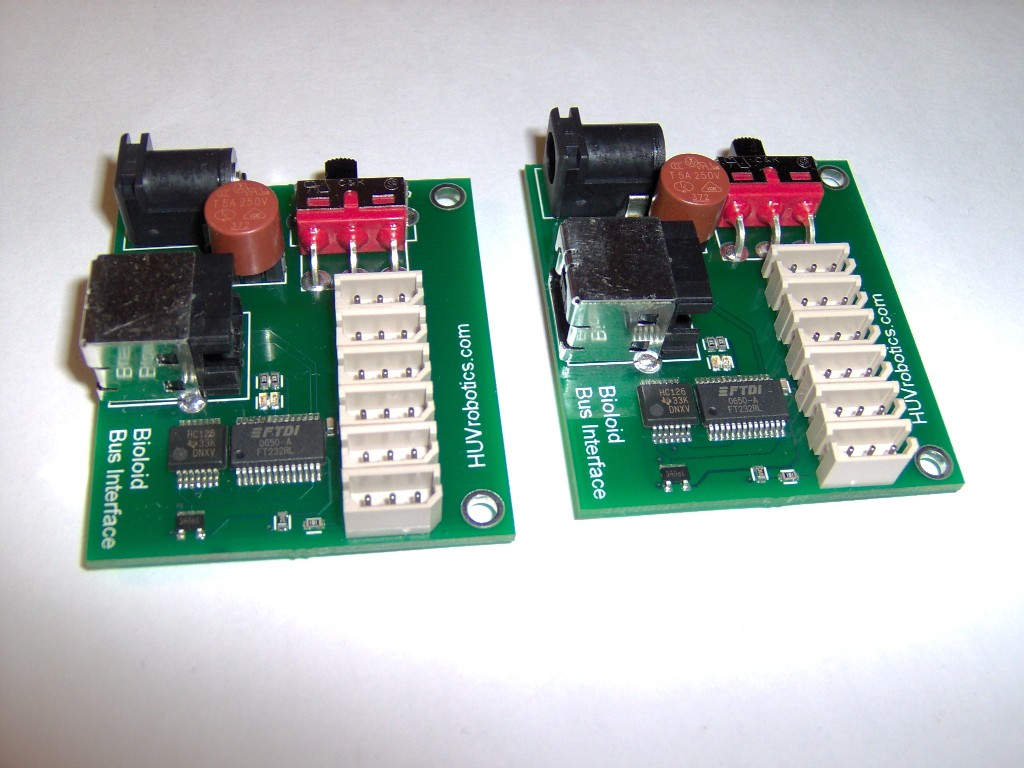
\includegraphics[width=0.5\textwidth]{img/busInterface.jpg}%
	\caption{Bioloid Bus Interface}
	\label{fig:busInterface}
\end{figure}
This board allows PC to communicate with Bioloid bus devices (e.g. Dynamixel AX-12) using a USB cable at speeds of up to 1.0 Mbps. In other words,
this simple device provides serial communication between the PC and the motors. It is also needed to provide voltage to the motors. We can not use it to power up the laser as the output voltage is too high and there is no voltage regulator.
\subsection{Laser Diode and Arduino Uno Board}
\begin{figure}
\centering
\begin{minipage}{.5\textwidth}
  \centering
  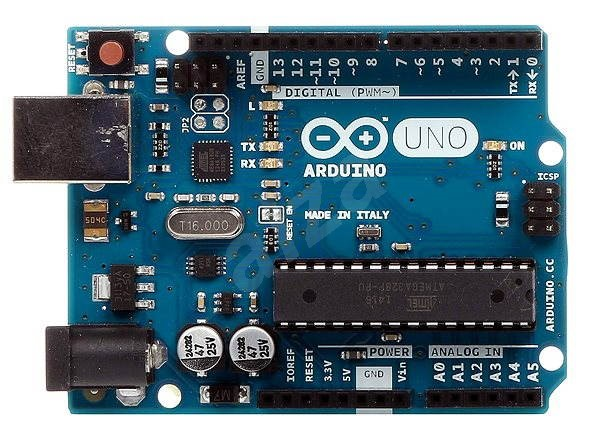
\includegraphics[width=\linewidth]{img/arduino.jpg}
  \captionof{figure}{Arduino Uno Board}
  \label{fig:arduino}
\end{minipage}%
\begin{minipage}{.5\textwidth}
  \centering
  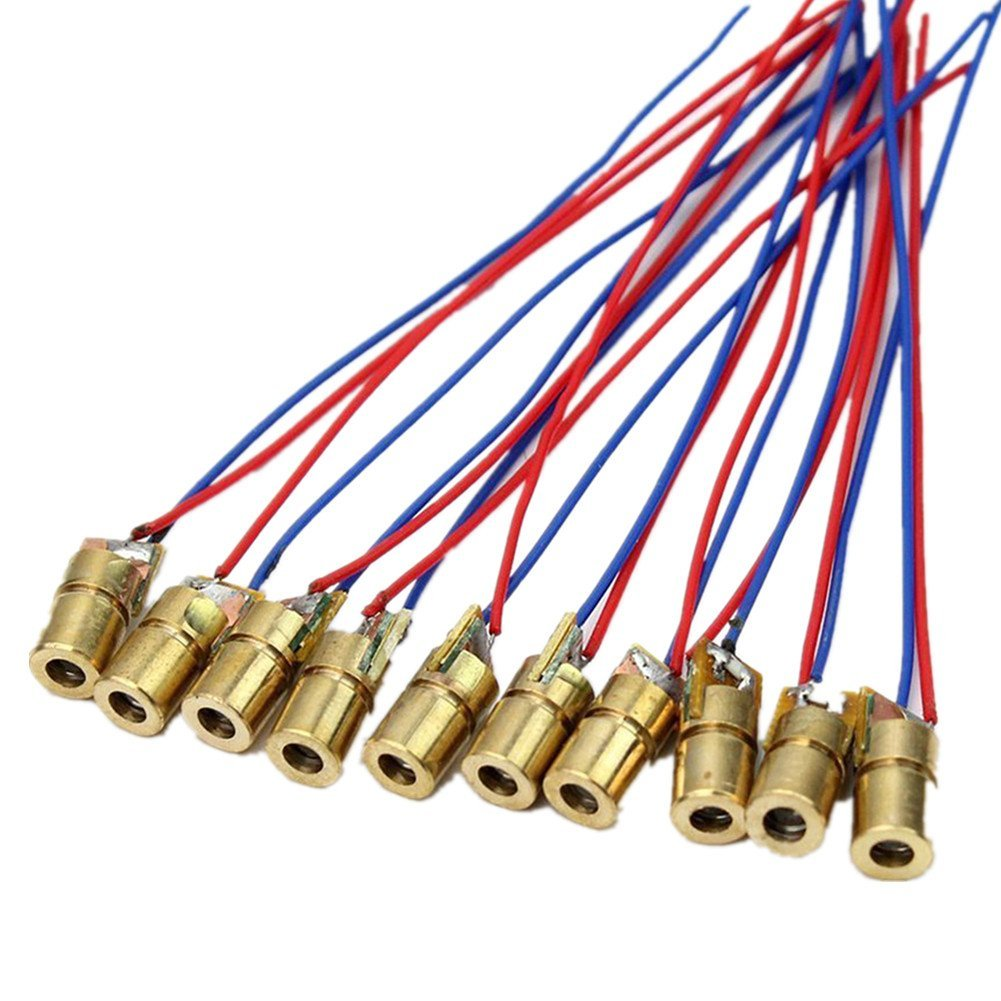
\includegraphics[width=.75\linewidth]{img/diode.jpg}
  \captionof{figure}{Laser Diodes}
  \label{fig:diode}
\end{minipage}
\end{figure}
We use a simple 5V red laser diode powered directly from an \emph{Arduino Uno Board}. We use that board because it provides a 5V output and thus is a simple and fast solution to power the laser up.
\subsection{Structural Parts}
Figures \ref{fig:axFrames} shows the plastic frames used to assemble the turret. Figures \ref{fig:axMounting1} and \ref{fig:axMounting2} shows how they are attached to the motor.
\begin{figure}
	\centering
	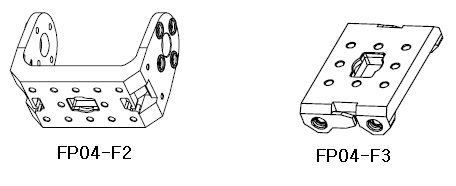
\includegraphics[width=\textwidth]{img/axFrames.png}%
	\caption{Plastic Frames}
	\label{fig:axFrames}
\end{figure}
\begin{figure}
	\centering
	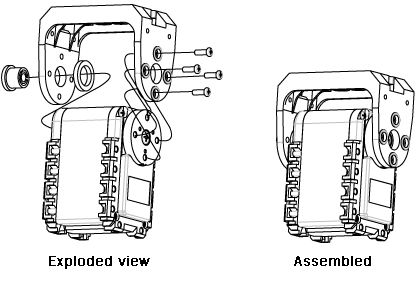
\includegraphics[width=\textwidth]{img/axMounting1.png}%
	\caption{Mounting F2 Frame}
	\label{fig:axMounting1}
\end{figure}
\begin{figure}
	\centering
	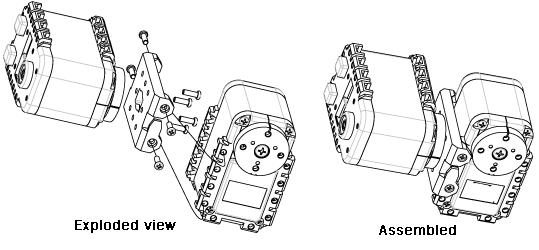
\includegraphics[width=\textwidth]{img/axMounting2.png}%
	\caption{Mounting F3 Frame}
	\label{fig:axMounting2}
\end{figure}
\section{Second Turret Model}\label{sec:turret64}
\begin{figure}
	\centering
	\includegraphics[width=\textwidth]{img/mx64Turret.png}%
	\caption{MX64 Turret}
	\label{fig:mx64Turret}
\end{figure}
As already mentioned, after we were able to get the best from the first model, we decided to base our system on a new and more powerful turret. In \ref{fig:mx64Turret} (DA SCATTARE) we can immediately see that there are some structural difference from the previous model, but those are already discussed in \ref{subs:secondModel}. Here, we want to discuss the new hardware, in particular motors and structural parts, which come from the ScorpionX MX-64 Robot Turret Kit by Interbotix \cite{MX64Turret}.
\subsection{Dynamixel MX-64T}
Quoting from \cite{web-MX64}:\\
\virgolette{\textit{The MX-64T Dynamixel Robot Servo Actuator is the newest generation of Robotis Dynamixel actuator; equipped with an onboard 32bit 72mhz Cortex M3, a contact-less magnetic encoder with 4x the resolution over the AX/RX series, and up to 3mpbs using the new TTL 2.0 bus. Each servo has the ability to track its speed, temperature, shaft position, voltage, and load. As if this weren't enough, the newly implemented PID control algorithm used to maintain shaft position can be adjusted individually for each servo, allowing you to control the speed and strength of the motor's response. All MX Series servos use 12v nominal voltage, so MX Dynamixels can be mixed without having to worry about separate power supplies. All of the sensor management and position control is handled by the servo's built-in microcontroller. This distributed approach leaves your main controller free to perform other functions.}}\\
So, we already know that those motors are more powerful than the ones used for the first model. Moreover, they are also compatible. The result is that we were able to use the same software interface written for the first turret without any issues, obtaining a more reliable model in term of accuracy, precision and trajectory smoothness. That confirms that we were doing things right also with the first turret, but we were facing its physical/hardware limitations. The results with the new turret immediately proved to be so good that we did not try to directly exploit and tune the more sophisticated functions offered by the new motors, such as built-in PID controllers or faster communication.
\subsection{Motor Specification}
\begin{figure}
	\centering
	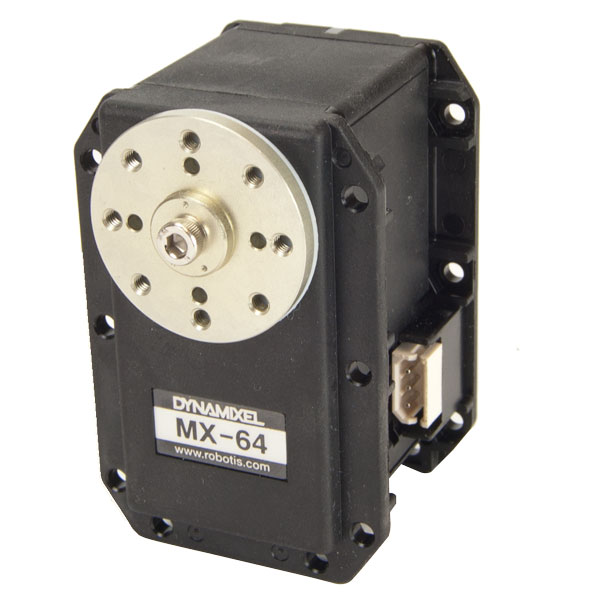
\includegraphics[width=0.5\textwidth]{img/mx64.jpg}%
	\caption{Dynamixel MX-64}
	\label{fig:mx64}
\end{figure}
From the full datasheet \cite{datasheet-MX64} we report only two important specifications:
\begin{itemize}
    \item \textbf{Resolution}: $0.088^{\circ}$;
    \item \textbf{Communication Speed}: 8000 bps $\sim$ 4.5 Mbps.
\end{itemize}
As we can see, the resolution of those servos is roughly 3 times better than the Dynamixel AX-12. This was enough to make the new turret perform perfectly for our needs using exactly the same approach we used to solve the issues explained in \ref{subs:firstModel:issues}
\subsection{Other Components}
Though we use a 3V green laser diode on that turret, the other components are the same: \emph{Bioloid Bus Interface} for communication and \emph{Arduino Uno Board} for powering the laser (that time from the 3.3V output).\\
The structural parts are provided together with the ScorpionX MX-64 Robot Turret Kit. Since the bracket of the tilt servo is too short, we had to mount the laser diode perpendicularly, obtaining the different structure already discussed. MAGARI FOTO DETTAGLIO LASER
\section{Arm IMU}
As explained in \ref{sec:1.2}, we needed an arm IMU device to reconstruct the direction of human pointing. First, we used the Myo Armband, \virgolette{\textit{a gesture recognition device worn on the forearm and manufactured by Thalmic Labs. The Myo enables the user to control technology wirelessly using various hand motions. It uses a set of electromyographic (EMG) sensors that sense electrical activity in the forearm muscles, combined with a gyroscope, accelerometer and magnetometer to recognize gestures.}}. Obviously, we were only interested only into the functions provided by gyroscope, accelerometer and magnetometer. We used such an expensive and mostly unnecessary device because it was what we already had.\\ Lately, we moved to a cheaper and more suitable device, the MetaMotionR board by Mbientlab, which can be mounted on a wrist band and provides a 9-axis IMU with Sensor Fusion. This is more convenient for our purposes, as it is easier to setup (it has a bluetooth driver for linux), more comfortable to wear (it is just like a watch) and also provides a LED for colour feedback and a small button (both are useful for our experiments and demos).
\begin{figure}
	\centering
	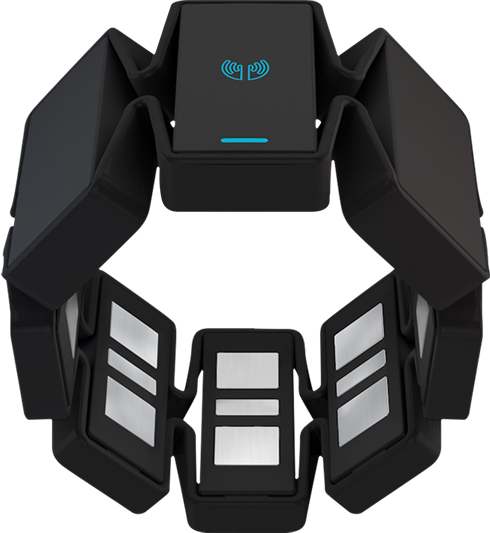
\includegraphics[width=0.5\textwidth]{img/myo.png}%
	\caption{Myo Armband}
	\label{fig:myo}
\end{figure}
\begin{figure}
	\centering
	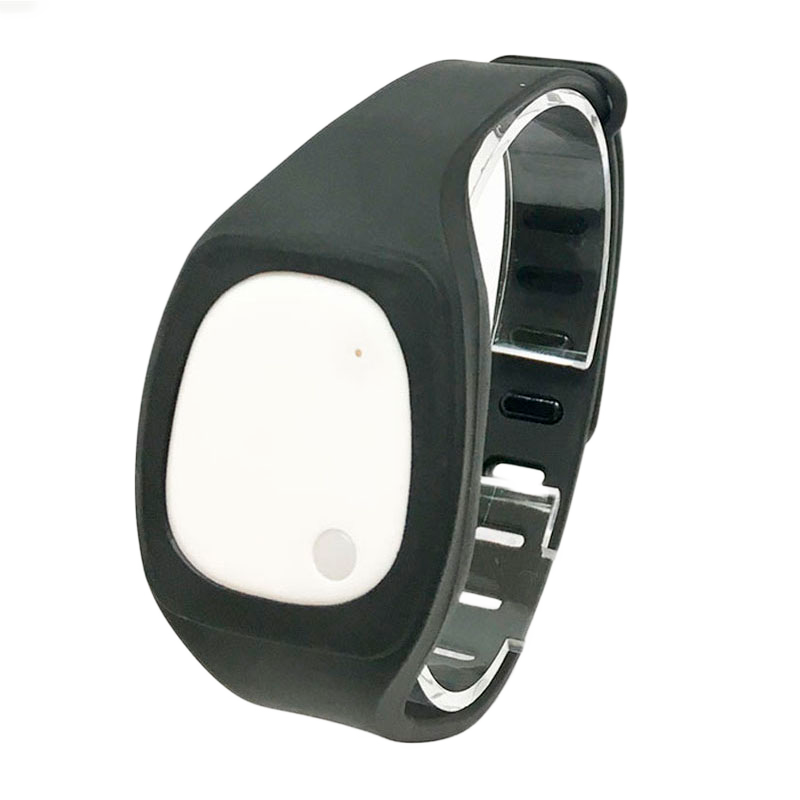
\includegraphics[width=0.5\textwidth]{img/rwristband.png}%
	\caption{MetaMotionR Wrist Band}
	\label{fig:rwristband}
\end{figure}
\section{Kobuki}
\virgolette{\textit{iClebo Kobuki is a low-cost mobile research base designed for education and research on state of art robotics. With continuous operation in mind, Kobuki provides power supplies for an external computer as well as additional sensors and actuators. Its highly accurate odometry, amended by our factory calibrated gyroscope, enables precise navigation.}} \cite{kobuki}.\\
As already stated, one of the main application of our system is ground robot navigation. We developed a couple of demo using the \emph{Kobuki}, a groud robot suitable for our purposes. Note that we actually use a \emph{TurtleBot2}, but only its structure (i.e. \emph{Kobuki} base plus mounting platform). For example, we do not exploit the \emph{kinect} camera provided with the \emph{Turtlebot2}. Its structure is perfectly suitable to mount our turret on top and thus demonstrate our system.
\begin{figure}
	\centering
	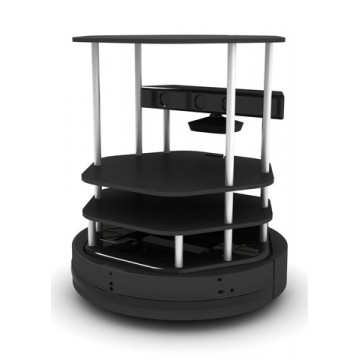
\includegraphics[width=0.5\textwidth]{img/turtlebot.jpg}%
	\caption{Turtlebot2 (with Kobuki base)}
	\label{fig:turtlebot}
\end{figure}